\documentclass{beamer}
\usetheme{Boadilla}
\usepackage{hyperref}
\usepackage{graphicx}
\usepackage{fancyvrb}
\usepackage{multicol}
\usepackage{subfig}
\usepackage{xcolor}
\usepackage{optparams}
\usepackage{xstring}
\usepackage[
    backend=biber, 
    natbib=true,
    style=numeric,
    sorting=none,
    style=verbose-ibid,
]{biblatex}
\addbibresource{citations.bib}
\usepackage{pgfpages}
\definecolor{ao(english)}{rgb}{0.0, 0.5, 0.0}
\definecolor{burgundy}{rgb}{0.5, 0.0, 0.13}
%\setbeameroption{show notes}
\setbeameroption{show notes on second screen=right}
%\setbeameroption{hide notes}

\def\footshortciteintern[#1][#2]#3{%
\ifx#1\empty 
% Nur Autor
\footnote{\citeauthor{#3}, \citeyear{#3}.}
\else
\ifx#2\empty
% Autor und Seite
\footnote{\citeauthor{#3}, \citeyear{#3}, #1.}
\else
% Autor, Seite und vgl.
\expandafter  
\footnote{\citeauthor{#3}, \citetitle{#3}, \citeyear{#3}, \citeurl{#3}.}
\fi
\fi
}
\newcommand*\footshortcite{%
\optparams{\footshortciteintern}{[\empty][\empty]}
}
\newcommand*\footmediumcite{%
\optparams{\footshortciteintern}{[][]}
}


\title{Nonstationary Gabor frames}
\author{Sevag Hanssian}
\date{January 28, 2021}
\institute{MUMT 622, Winter 2021}
\setbeamertemplate{navigation symbols}{}

\begin{document}

\begin{frame}
\maketitle
\end{frame}

\begin{frame}
	\frametitle{Nonstationary Gabor frames}
	\begin{itemize}
		\item[2002] Multiple Gabor frame system for varying time-frequency resolution analysis of music\footfullcite{doerflerphd}
		\item[2009] Nonstationary Gabor frames document in LTFAT\footcite{jaillet}
		\item[2011] \textbf{Theory, implementation and applications of nonstationary Gabor frames}\footcite{balazs}
	\end{itemize}
\end{frame}

\note{
	\begin{itemize}
		\item
			this is not a strict timeline or exhaustive literature review, but some interesting ``family of papers''
		\item
			Monika D{\"o}rfler's PhD dissertation on gabor, varying TF resolution, music
		\item
			frame theory led to a serious solution for a practical, invertible CQT
	\end{itemize}
}

\begin{frame}
	\frametitle{Nonstationary Gabor frames}
	\begin{quote}
		The definition of multiple Gabor frames, which is comprehensively treated in [D{\"o}rfler 2002], provides Gabor frames with analysis techniques with multiple resolutions.\\
		\vspace{0.5em}
		The nonstationary Gabor frames (see [Jaillet 2009], [Balazs 2011] for their definition and implementation)  are a further development; they fully exploit theoretical properties of the analysis and synthesis operator, and extend the \textbf{painless} case... they provide for a class of FFT-based algorithms [...] together with perfect reconstruction formulas\footfullcite{adaptivecqt}
	\end{quote}
\end{frame}

\note{
	\begin{itemize}
		\item
			bolded painless because it's an interesting word - i will cover it later
	\end{itemize}
}

\begin{frame}
	\frametitle{Review: Gabor frames}
	Gabor's 1946 ``Theory of Communication''\footfullcite{gabor1946}:
	\begin{enumerate}
		\item
			First introduction of the time-frequency uncertainty principle
		\item
			Proposed that any signal can be chopped up and windowed with Gaussian functions to minimize TF uncertainty
	\end{enumerate}
	    \[ \sigma_{t}\sigma_{f} \ge \frac{1}{4\pi},\qquad\Delta t\Delta f \ge 1 \]
	\begin{figure}
		\vspace{-1.5em}
		\centering
		\subfloat[Max signal localization in TF: rectangles of size $\Delta t\Delta f = 1$]{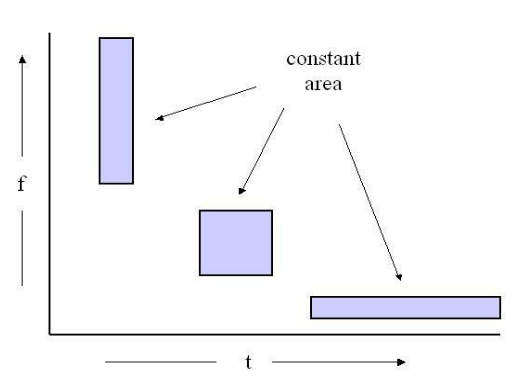
\includegraphics[width=4.5cm]{./tf-resolution.png}}
		\hspace{2.5em}
		\subfloat[Change TF tiling by modifying Gaussian]{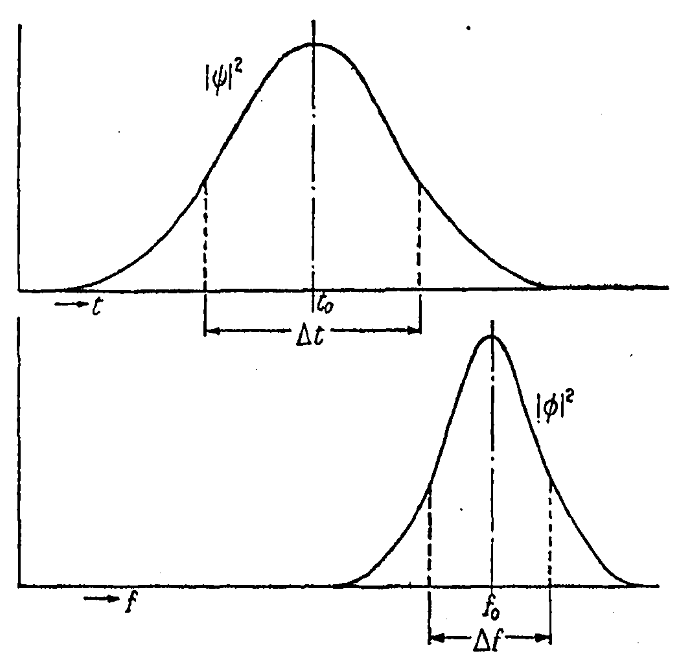
\includegraphics[width=3.5cm]{./gabor4.png}}
	\end{figure}
\end{frame}

\note{
	\begin{itemize}
		\item
			this material builds on the material from my last presentation
		\item
			start with the refresher
		\item
			recall that we are constrained to rectangles of this area
	\end{itemize}
}

\begin{frame}
	\frametitle{Review: fixed TF resolution STFT}
	MATLAB STFT with gausswin (i.e. Gabor transform)
	\begin{figure}
		\centering
		\subfloat[small window (128)]{{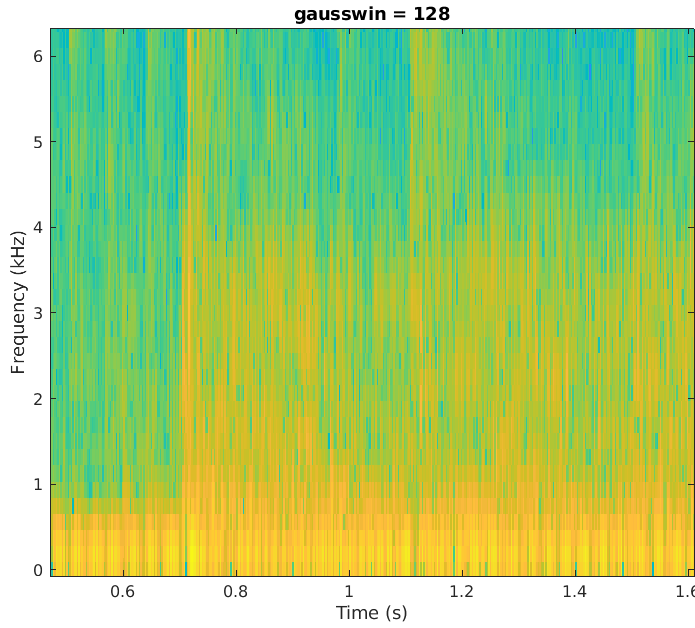
\includegraphics[width=5.04cm]{./gaborstft_small_zoomed.png} }}
		\subfloat[big window (16384)]{{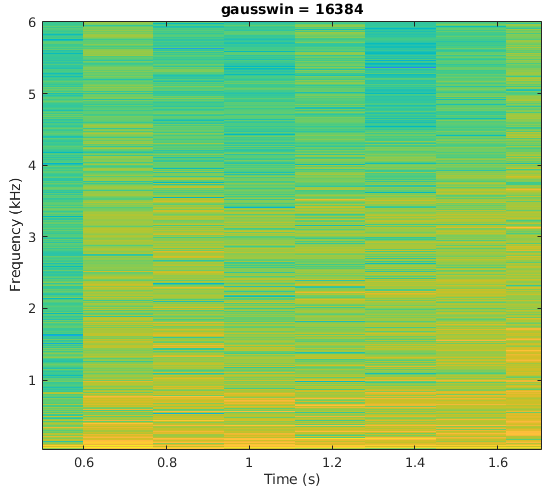
\includegraphics[width=5.1cm]{./gaborstft_big_zoomed.png} }}
		\caption{Good time resolution versus good frequency resolution}
	\end{figure}
\end{frame}

\begin{frame}
	\frametitle{Fixed TF resolution for music}
	\begin{figure}
		\centering
		\subfloat{{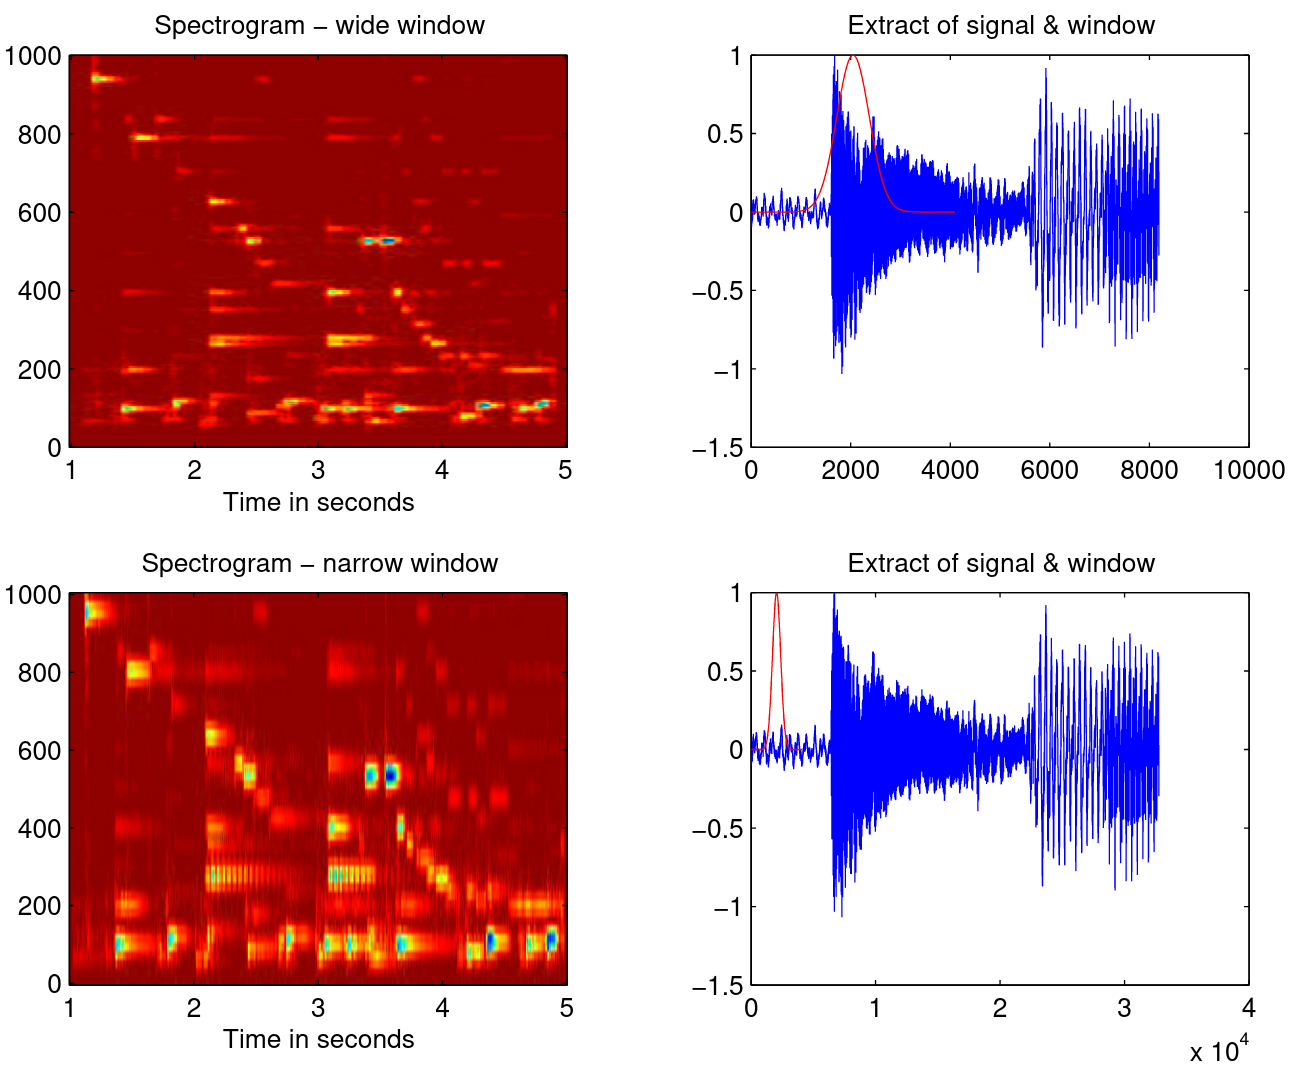
\includegraphics[width=6.5cm]{./tf_tradeoff_dorfler.png} }}
		\subfloat{{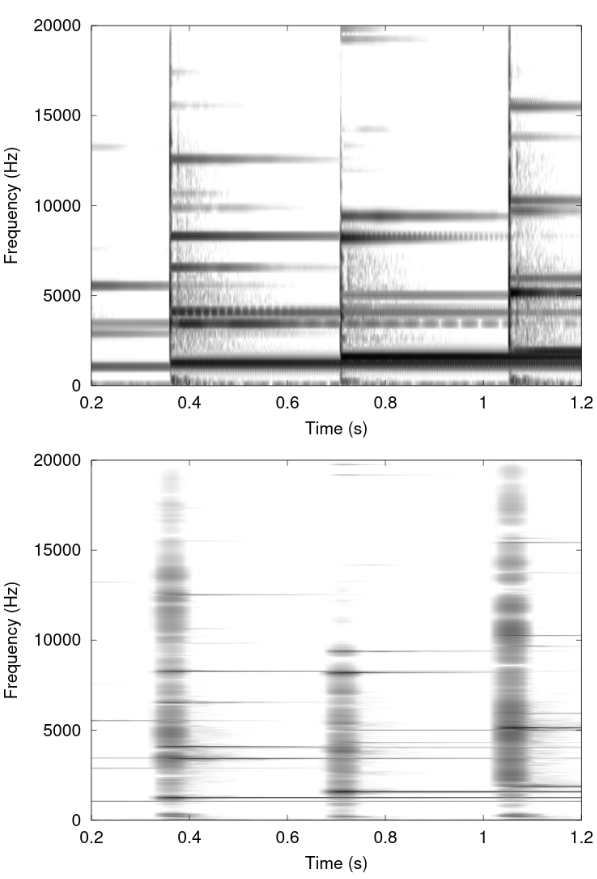
\includegraphics[width=3.7cm]{./tf_tradeoff_balasz1.png} }}
		\caption{Two windows for music signal\footshortcite{doerflerphd} and glockenspiel\footshortcite{jaillet}}
	\end{figure}
\end{frame}

\begin{frame}
	\frametitle{Stationary Gabor frames}
	In the standard Gabor analysis, same window function (aka Gabor atom, Gabor function) is shifted in time to cover entire signal\footshortcite{adaptivecqt}:
	\[ g_{\tau, \omega}(t) = g(t - \tau)e^{2\pi i t \omega} \]

	\begin{columns}
           \column{0.5\linewidth}
		\begin{quote}
			We will indicate such a frame as \textit{stationary}, since the window used for time-frequency shifts does not change and the time-frequency shifts form a lattice of $a\text{ }x\text{ }b$
		\end{quote}
          \column{0.5\linewidth}
		\hspace{-2em}
		%\vspace{6em}
	    \centering
	     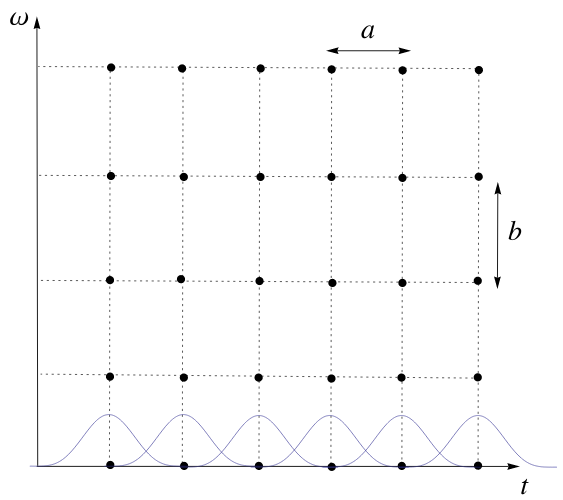
\includegraphics[width=4cm]{stationarygabor.png}
        \end{columns} 
\end{frame}

\note{
	\begin{itemize}
		\item
			Last presentation, I didn't call it stationary - only ``gabor frame'' alone
		\item
			until the non-stationary variant was created, there was no need to call the original stationary
	\end{itemize}
}

\begin{frame}
	\frametitle{Musical justification for Constant-Q Transform}
		Constant-Q transform for music analysis\footfullcite{jbrown}, \footfullcite{msp}:
		\begin{enumerate}
			\item
				Harmonics of the fundamental have consistent spacing in the log scale -- the constant pattern\\
				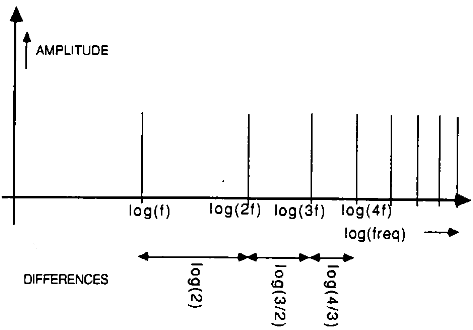
\includegraphics[height=3cm]{./logharmonic.png}
			\item
				Log-frequency spectra, demonstrating the constant pattern for harmonics, would be more useful in musical tasks
		\end{enumerate}
\end{frame}

\note{
	\begin{itemize}
		\item
			judith brown, MSP (of miller s puckette fame)
		\item
			constant-Q transform was known about before Gabor frames - like i discussed with prof
		\item
			tasks such as instrument identification by timbre, etc.
		\item
			also lines up with pitch perception as pattern recognition
	\end{itemize}
}

\begin{frame}
	\frametitle{Violin: DFT vs. CQT}
	\begin{figure}
		\vspace{-1em}
		\centering
		\subfloat[Constant Q transform]{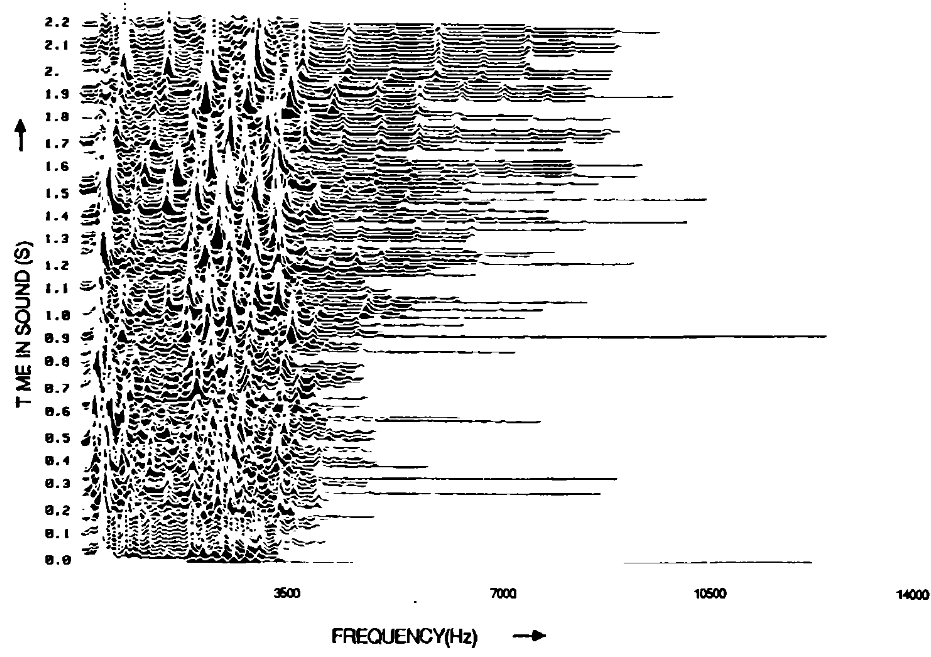
\includegraphics[height=3.75cm]{./violindft.png}}
		\subfloat[Discrete Fourier Transform]{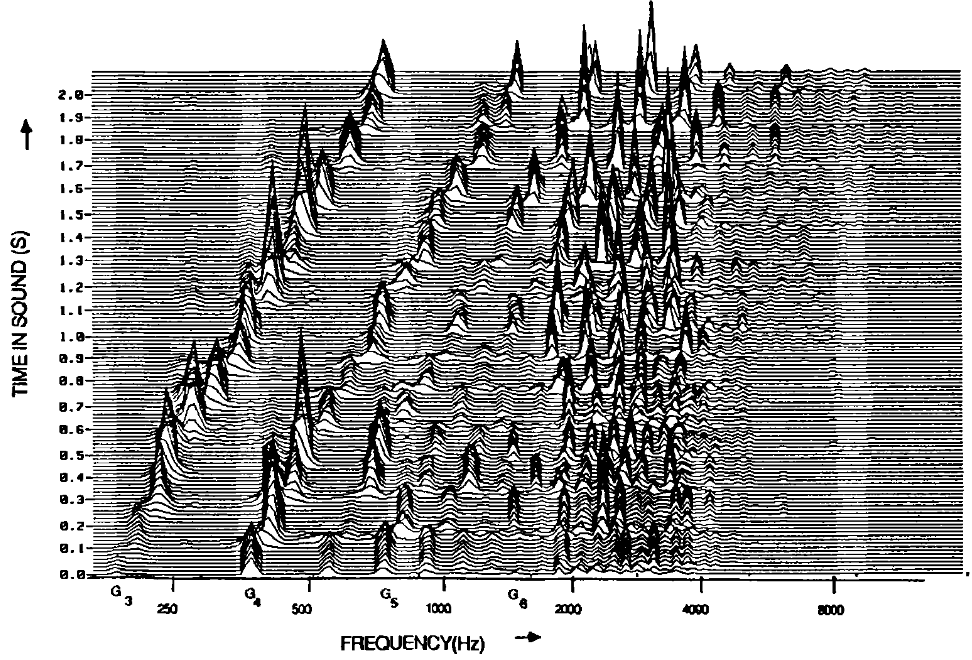
\includegraphics[height=3.75cm]{./violincqt.png}}
		\caption{Violin playing diatonic scale, $G_{3} \text{(196Hz)} - G_{5} \text{(784Hz)}$\footshortcite{jbrown}}
	\end{figure}
\end{frame}

\note{
	\begin{itemize}
		\item
			Not explicitly named as an STFT but we know it is
		\item
			we can see note changes clearly, the fundamental, and even the formant in 3000hz region
	\end{itemize}
}

\begin{frame}
	\frametitle{Constant-Q Transform}
	``Constant ratio of frequency to frequency resolution'': $\frac{f}{\delta f} = Q$
	\begin{figure}
		\vspace{-1em}
		\centering
		\subfloat[Properties of DFT, CQT]{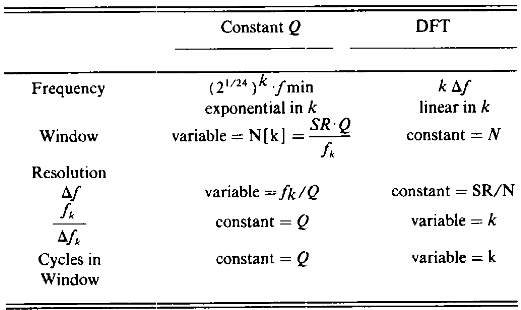
\includegraphics[height=3.5cm]{./dftvcqt.png}}
		\subfloat[Window sizes for CQT]{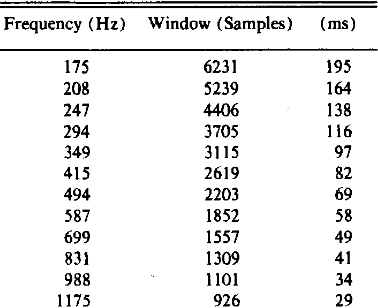
\includegraphics[height=3.5cm]{./qwindowchanges.png}}
	\end{figure}
	Computed with windowed DFT where window changes with frequency to maintain Constant-Q\footshortcite{jbrown} -- \textbf{non-invertible!}:
	\[ \text{window len } N[k] = \frac{f_{s}}{f_{k}}Q, W[k, n] = \alpha + (1 - \alpha)\cos(\frac{2\pi n}{N[k]}) \]
\end{frame}

\note{
	\begin{itemize}
		\item
			meanwhile the linear spacing of conventional DFT leads to a pattern that varies with the harmonic -- making it harder to identify 
		\item
			in linear DFT, pattern of harmonic spacing changes with frequency
	\end{itemize}
}

\begin{frame}
	\frametitle{Musical justification for nonstationary Gabor frames}
	\begin{quote}
		In the case of music signals, for example, transients are important for several reasons. They give important cues for onset timing, and they carry information about instrument timbre. As another example, in low-frequency regions, very fine frequency resolution is required, because notes in this region lay the harmonic basis, musically speaking.\\
		\vspace{0.4em}
		In order to achieve a setting adapted to music as discussed above, it will be necessary to use wider windows with good frequency concentration in low-frequency regions, whereas in the high-pass regions, where mainly transients and broadband signals components occur, rather short windows, which don't have to be very localised in frequency, will be of use \footshortcite{doerflerphd}
	\end{quote}
\end{frame}

\note{
	\begin{itemize}
		\item
			similar motivation, except Dorfler et all are using this motivation to drive mathematical theory
		\item
			the lack of theory didn't affect the evolution, or desire, for the CQT
	\end{itemize}
}

\begin{frame}
	\frametitle{Nonstationary Gabor frames}
	\textbf{PAINLESS}
	In the standard Gabor analysis, same window function (aka Gabor atom, Gabor function) is shifted in time to cover entire signal\footfullcite{adaptivecqt}:
	\[ g_{\tau, \omega}(t) = g(t - \tau)e^{2\pi i t \omega} \]

	\begin{columns}
           \column{0.5\linewidth}
		\begin{quote}
			We will indicate such a frame as \textit{stationary}, since the window used for time-frequency shifts does not change and the time-frequency shifts form a lattice of $a\text{ }x\text{ }b$
		\end{quote}
          \column{0.5\linewidth}
		\hspace{-2em}
		%\vspace{6em}
	    \centering
	     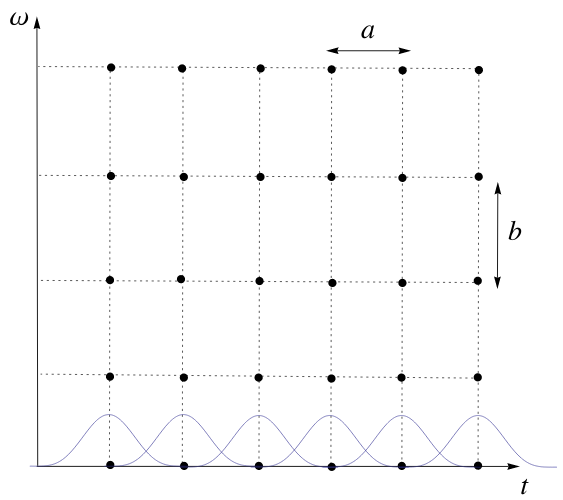
\includegraphics[width=4cm]{stationarygabor.png}
        \end{columns} 
\end{frame}

\note{
	\begin{itemize}
	\item
		so with NSGT now, the CQT is revisited and formulated in an invertible way
	\end{itemize}
}

\begin{frame}
	\frametitle{CQT implementations}
	\begin{itemize}
		\item[2012] Invertible, realtime CQT based on nonstationary Gabor transform\footcite{rtcqt}
		\item[2018] CQT/ICQT added in MATLAB Wavelet Toolbox\footcite{matlabcqt}
	\end{itemize}
	mention alternative: https://librosa.org/doc/latest/generated/librosa.cqt.html
	2010 klapuri
\end{frame}

\end{document}
